\documentclass{beamer}
\usetheme{CambridgeUS}
\usepackage[brazil]{babel}
\usepackage[utf8]{inputenc}

\title{Aprendizado Semi-Supervisionado Baseado em Grafos}
\subtitle{Seminário da Matéria SCC5882 \\ Professores: Dr. Zhao Liang e Dr. Alneu de Andrade Lopes}
\author{Aluno: Renato Fabbri}

%\date
\begin{document}
  \frame{\titlepage}
  \section{Apresentação}
    \subsection{Sumário}
      \frame{\tableofcontents}
    \subsection{Resumo}
      \frame
      {
        \frametitle{Resumo}
        \begin{figure}[!h]
          \begin{center}
                  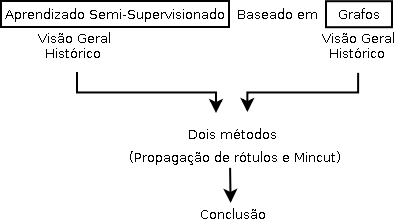
\includegraphics[width=0.75\textwidth]{Diagram1}
          \end{center}
    %         \caption{Gráfico Curioso}
        \end{figure}
      }

  \section{Introdução}
    \frame{\tableofcontents[current]}

    \subsection{Aprendizado Semi-Supervisionado}
      \frame
      {
        \frametitle{A - Definições (1)}
        \begin{itemize}
          \item <1-> Aprendizado Supervisionado - treinamento somente com os dados rotulados
          \item <2-> Aprendizado não Supervisionado - utilizados somente dados não rotulados
          \item <3-> Aprendizado Semi-Supervisionado - utilização tanto dos dados rotulados quanto dos não rotulados.
        \end{itemize}
      }

      \frame
      {
        \frametitle{A - Definições (2)}
        \begin{itemize}
          \item <1-> Classificação Semi-Supervisionada, CSS. (Clusterização forçada não é foco)
          \item <2-> Indutivo e Transdutivo.
        \end{itemize}
      }

      \frame
      {
        \frametitle{A - Interesse}
        \begin{itemize}
          \item <1-> Criança aprendendo as coisas (animais).
          \item <2-> Dados rotulados podem ser poucos ou custosos.
        \end{itemize}
      }
          
      \frame
      {
        \frametitle{A - Caso 1}
        \begin{figure}[!h]
        \begin{center}
                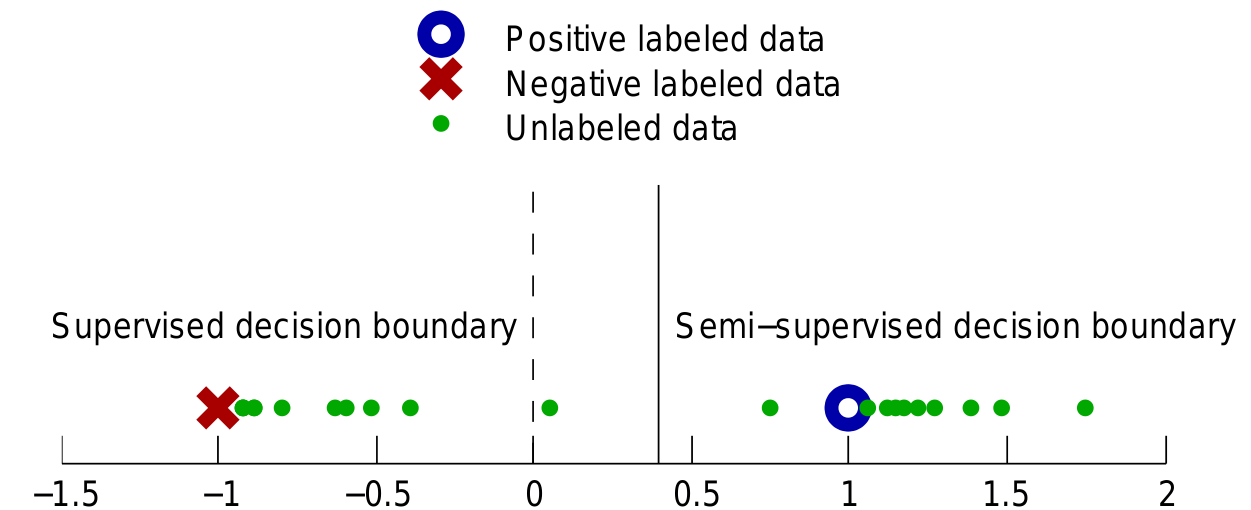
\includegraphics[width=0.75\textwidth]{ssl-help}
        \end{center}
        \caption{Forma em que a CSS auxilia na classificação. Fonte: Zhu, X. and Lafferty, J. and Rosenfeld, R., 2005}
      \end{figure}
      }

      \frame
      {
        \frametitle{A - Caso 2}
        \begin{figure}[!h]
        \begin{center}
                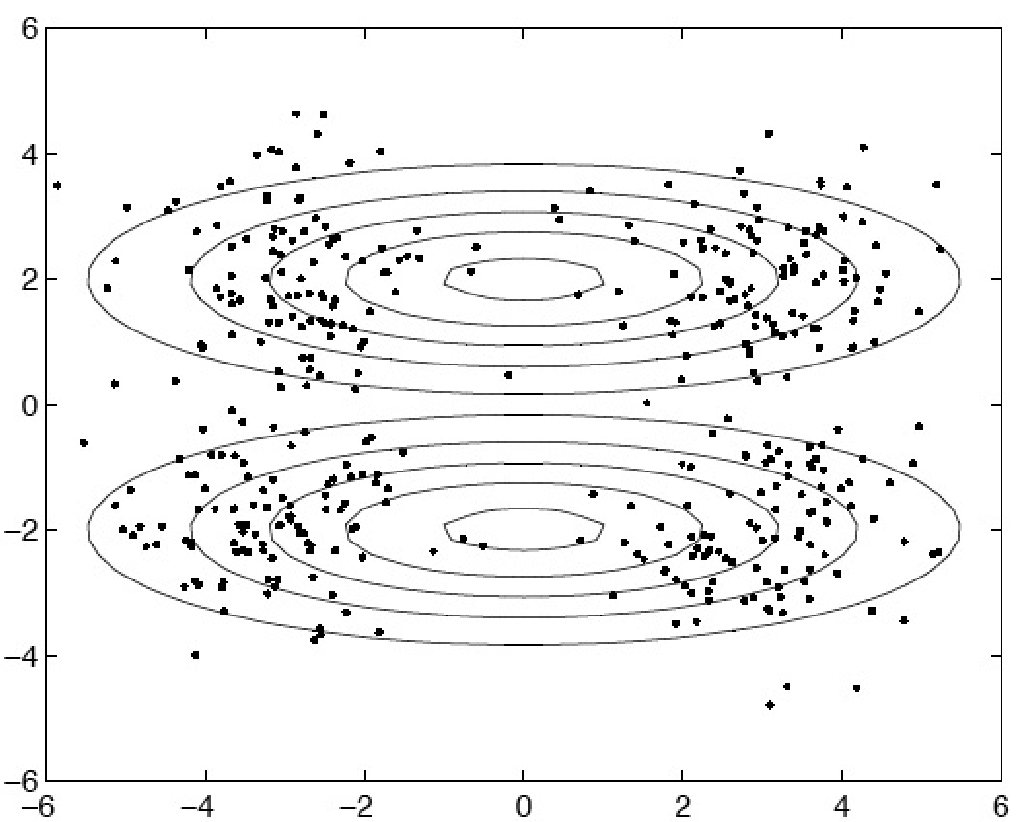
\includegraphics[width=0.75\textwidth]{ssl-nhelp}
        \end{center}
        \caption{Forma em que a CSS atrapalha na classificação. Fonte: Müller, K. R. and Zien, A., 2008}
      \end{figure}
      }

      \frame
      {
        \frametitle{A - Breve Histórico}
        \begin{itemize}
          \item <1-> Primeiros: Modelos de Mistura.
          \item <2-> Primeiros: Self-Training (self-teaching e bootstrapping).
          \item <3-> Mais recentes: Co-training e SVM transdutivo.
          \item <4-> Mais recentes: Métodos baseados em grafos.
        \end{itemize}
      }

    \subsection{Grafos e Redes Complexas}
      \frame{\tableofcontents[current]}

      \frame
      {
        \frametitle{G \& RC - Definição (1)}
        \begin{itemize}
          \item <1-> Conjunto de objetos, alguns ligados.
          \item <2-> Objetos $\rightarrow$ nós ou vértices. Ligações $\rightarrow$ arestas.
          \item <3-> Visualmente $\rightarrow$ pontos e linhas.
        \end{itemize}
      }

      \frame
      {
        \frametitle{G \& RC - Variações}
        \begin{itemize}
          \item <1-> Arestas Direcionadas.
          \item <2-> Pesos nas arestas.
          \item <3-> Mais de um tipo de aresta.
          \item <4-> Atributos quaisquer associados às arestas e aos nós.
        \end{itemize}
      }

      \frame
      {
        \frametitle{G \& RC - Exemplos Clássicos}
        \begin{itemize}
          \item <1-> Regular.
          \item <2-> Completo (\emph{click}).
          \item <3-> Conectado.
          \item <4-> Randômico.
          \item <5-> trivial, nulo, etc.
        \end{itemize}
      }

      \frame
      {
        \frametitle{G \& RC - Medidas mais Comuns}
        \begin{itemize}
          \item <1-> Grau.
          \item <2-> Força.
          \item <3-> Entrada e Saída.
        \end{itemize}
      }

      \frame
      {
        \frametitle{G \& RC - Rede Complexa}
        \begin{itemize}
          \item Grafo de grandes dimensões.

          \item Casos triviais - RC randômica e regular.
        \end{itemize}
      }

      \frame
      {
        \frametitle{G \& RC - Breve Histórico}
        \begin{itemize}
          \item <1-> Euler - ”Konigsberg Bridge problem”.
          \item <2-> Cayley - Química.
          \item <3-> "Grafo" Nature - Silvester 1878.
          \item <4-> Grafos, topologia, álgebra - Lei de Kirchoff
          \item <5-> Teorias probabilísticas
          \item <6-> RC naturais - propriedades não triviais - LE, PM.
          \item <7-> Neurociência, Física, Linguística, Computação, etc.
        \end{itemize}
      }

  \section{Aprendizado Semi-Supervisionado em Grafos}
    \frame{\tableofcontents[current]}

    \frame
    {
      \frametitle{CSS em G}
      \begin{itemize}
        \item Algorítmo de regularização.
        \item Mincut
        \item Propagação de Rótulo.
        \item Modelos de Mistura.
        \item Máxima Entropia.
        \item ETC.
      \end{itemize}
    }

    \subsection{Propagação de Rótulo}
      \frame{\tableofcontents[current]}

      \frame
      {
        \frametitle{PR - Concepção}
        \begin{itemize}
          \item <1-> Vizinho mais próximo $\rightarrow$ propaga mais fácil.
          \item <2-> Rótulos fixos nos rotulados de antemão.
          \item <3-> Estes "emanam" os seus rótulos.
        \end{itemize}
      }

      \frame
      {
        \frametitle{Convenções e Exposição do Problema (1)}
        \begin{itemize}
          \item <1-> ${(x_1,y_1)...(x_l,y_l)}$ os dados rotulados.
          \item <2-> $y \in {1...C}$ com $C$ o número de classes.
          \item <3-> ${x_{l+1}...x_{l+u}}$.
          \item <4-> Geralmente $l \ll u$.
          \item <5-> Seja $n = l + u$
          \item <6-> L e U denotam os dados rotulados e não rotulados, respectivamente
        \end{itemize}
      }

      \frame
      {
        \frametitle{Convenções e Exposição do Problema (2) - Notas}
        \begin{itemize}
          \item <1-> Cada classe de C presente em ao menos 1 elemento.
          \item <2-> Método Transdutivo.
        \end{itemize}
      }

      \frame
      {
        \frametitle{Convenções e Exposição do Problema (3) - Obtenção do Grafo}
        \begin{itemize}
          \item <1-> Completo.
          \item <2-> $w_{ij} = exp( -\frac{\| x_i - x_j \|^2}{\alpha^2} )$
          \item <3-> $\alpha$ é um \emph{hiperparâmetro}
        \end{itemize}
      }  

      \frame
      {
        \frametitle{Convenções e Exposição do Problema (4) - Transição}
        \begin{itemize}
          \item <1-> $P_{ij}$ é a probabilidade de transição do nó $i$ para o nó $j$ (passagem do rótulo)
          \item <2-> $P_{ij} = P(i \rightarrow j) = \frac{w_{ij}}{\sum_{k=1}^{n}w_{ik}}$
        \end{itemize}
      }

      \frame
      {
        \frametitle{Convenções e Exposição do Problema (5) - Últimas Definições}
        \begin{itemize}
          \item <1-> Matriz de rótulos $Y_L$, $l \times C$, cuja \emph{iésima} linha possui $1$ na coluna correspondente à classe do dado $x_i$.
          \item <2-> $f$ uma matriz $n \times C$ em que cada linha pode ser interpretada como uma distribuição de probabilidade sobre os rótulos.
        \end{itemize}
      }

      \frame
      {
        \frametitle{Convenções e Exposição do Problema (5) - Tarefa!}
          A tarefa consiste em computar os rótulos dos nós todos (na verdade somente dos não rotulados)

      }

      \frame
      {
        \frametitle{O Algoritmo de Propagação de Rótulo}
        \begin{itemize}
          \item Propague $f \leftarrow Pf$. (todos os nós propagam o seu rótulo para os seus vizinhos)
          \item Mantenha os dados rotulados iniciais $f_L = Y_L$. (assegura que os rótulos dos nós inicialmente rotulados não sejam sobrescritos)
          \item Repita do passo 1 até que o algoritmo convirja.
        \end{itemize}
      }

      \frame
      {
        \frametitle{PR - Convergência (1)}
          \begin{equation}
            f = \binom{f_L}{f_U}
          \end{equation}

          \begin{equation}
            \begin{bmatrix}
              P_{LL} & P_{LU}
              \\P_{UL} & P_{UU}
            \end{bmatrix}
          \end{equation}

          \begin{equation} \label{eq:inicio}
            f_U \leftarrow P_{UU}f_U + P_{UL}Y_L
          \end{equation}

          \begin{equation}
            f_u = \lim_{n \rightarrow \infty}[(P_{UU})^n f_U^0 + (\sum_{i=1}^{n}(P_{UU})^{(i-1)})P_{UL}Y_L]
          \end{equation}
      }

      \frame
      {
        \frametitle{PR - Convergência (2)}
          \begin{equation}
            f_u = \lim_{n \rightarrow \infty}[(P_{UU})^n f_U^0 + (\sum_{i=1}^{n}(P_{UU})^{(i-1)})P_{UL}Y_L]
          \end{equation}

          \begin{equation}
            (P_{UU})^n f_U^0 \rightarrow 0
          \end{equation}

          \begin{equation}
            \exists \; \gamma < 1 : \sum_{j = 1}^u(P_{UU})_{ij} \leq \gamma, \forall i = 1...u
          \end{equation}

Portanto:
\begin{equation}
  \sum_j(P_{UU})_{ij}^n \leq \gamma^n
\end{equation}

Então:

\begin{equation}
  f_u = (I - P_{UU})^{-1}P_{UL}Y_{L}
\end{equation}
      }

      \frame
      {
        \frametitle{PR - Exemplo 1 (1)}
        \begin{figure}[!h]
          \begin{center}
                  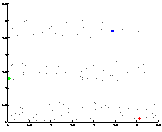
\includegraphics[width=0.75\textwidth]{prop1-dados}
          \end{center}
            \caption{Dados originais, 3 rotulados, 178 não rotulados.}
        \end{figure}
      }

      \frame
      {
        \frametitle{PR - Exemplo 1 (2)}
        \begin{figure}[!h]
          \begin{center}
                  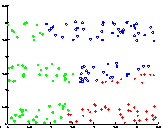
\includegraphics[width=0.75\textwidth]{prop1-dados-knn}
          \end{center}
            \caption{Dados rotulados utilizando-se knn.}
        \end{figure}
      }

      \frame
      {
        \frametitle{PR - Exemplo 1 (3)}
        \begin{figure}[!h]
          \begin{center}
                  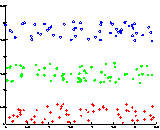
\includegraphics[width=0.75\textwidth]{prop1-dados-rotu}
          \end{center}
            \caption{Dados rotulados utilizando propagação de rótulos.}
        \end{figure}
      }


      \frame
      {
        \frametitle{PR - Exemplo 2 (1)}
        \begin{figure}[!h]
          \begin{center}
                  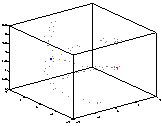
\includegraphics[width=0.75\textwidth]{prop2-dados}
          \end{center}
            \caption{Dados originais, 2 rotulados, 184 não rotulados.}
        \end{figure}
      }

      \frame
      {
        \frametitle{PR - Exemplo 1 (2)}
        \begin{figure}[!h]
          \begin{center}
                  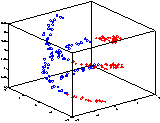
\includegraphics[width=0.75\textwidth]{prop2-dados-knn}
          \end{center}
            \caption{Dados espiralados rotulados utilizando-se knn.}
        \end{figure}
      }

      \frame
      {
        \frametitle{PR - Exemplo 1 (2)}
        \begin{figure}[!h]
          \begin{center}
                  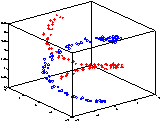
\includegraphics[width=0.75\textwidth]{prop2-dados-rotu}
          \end{center}
            \caption{Dados espiralados rotulados utilizando propagação de rótulos.}
        \end{figure}
      }

    \subsection{Mincut}
      \frame
      {
        \frametitle{Mincut - Concepção}
        \begin{itemize}
          \item Objetos parecidos devem ficar juntos.
          \item Seccionamento por separações de custos mínimos.
        \end{itemize}
      }

      \frame
      {
        \frametitle{Mincut - Convenções e Exposição do Problema}
        \begin{itemize}
          \item <1-> rotulados $L$ e não rotulados $U$.
          \item <2-> $L_+$ os positivos; $L_-$ os negativos.
          \item <3-> $v_+$ e $v_-$
        \end{itemize}
      }

      \frame
      {
        \frametitle{O Algoritmo de Propagação de Mincut}
        \begin{itemize}
          \item $G = (V,E)$, onde $V = L \cup U$ e $E \subseteq V \times V$
          \item $e \in E$ é associado um peso $w(e)$
          \item $w(v_1,v_2) = \infty, \forall \; v_1,v_2 \in L_+$ e $w(v_1,v_2) = \infty, \forall \; v_1,v_2 \in L_-$.
          \item Função de atribuição de pesos, denotada por $w$.
          \item Determinamos o conjunto de arestas com a menor soma de pesos que, se removidas, separam todos os $v_+$ dos $v_-$. (Corte mínimo)
          \item Por fim, rotulamos como positivos todos os vértices em $V_+$ e como negativos todos os vértives em $V_-$.
        \end{itemize}
      }

      \frame
      {
        \frametitle{Calibragem do Mincut}
        \begin{itemize}
          \item $w$ é sem dúvida o crucial neste algorítmo.
          \item {\bf Mincut-3}
          \item {\bf Mincut-$\delta$}, {\bf Mincut-$\delta_0$}, {\bf Mincut-$\delta_\frac{1}{2}$}, {\bf Mincut-$\delta_{opt}$}
        \end{itemize}
      }

      \frame
      {
        \frametitle{Mincut - Problemas}
        \begin{itemize}
          \item Difícil Calibragem.
          \item Casos de poucos exemplos rotulados
        \end{itemize}
      }

    \frame
    {
      \frametitle{Mincut - Desempenho Comparativo (1)}
      \begin{figure}[!h]
        \begin{center}
                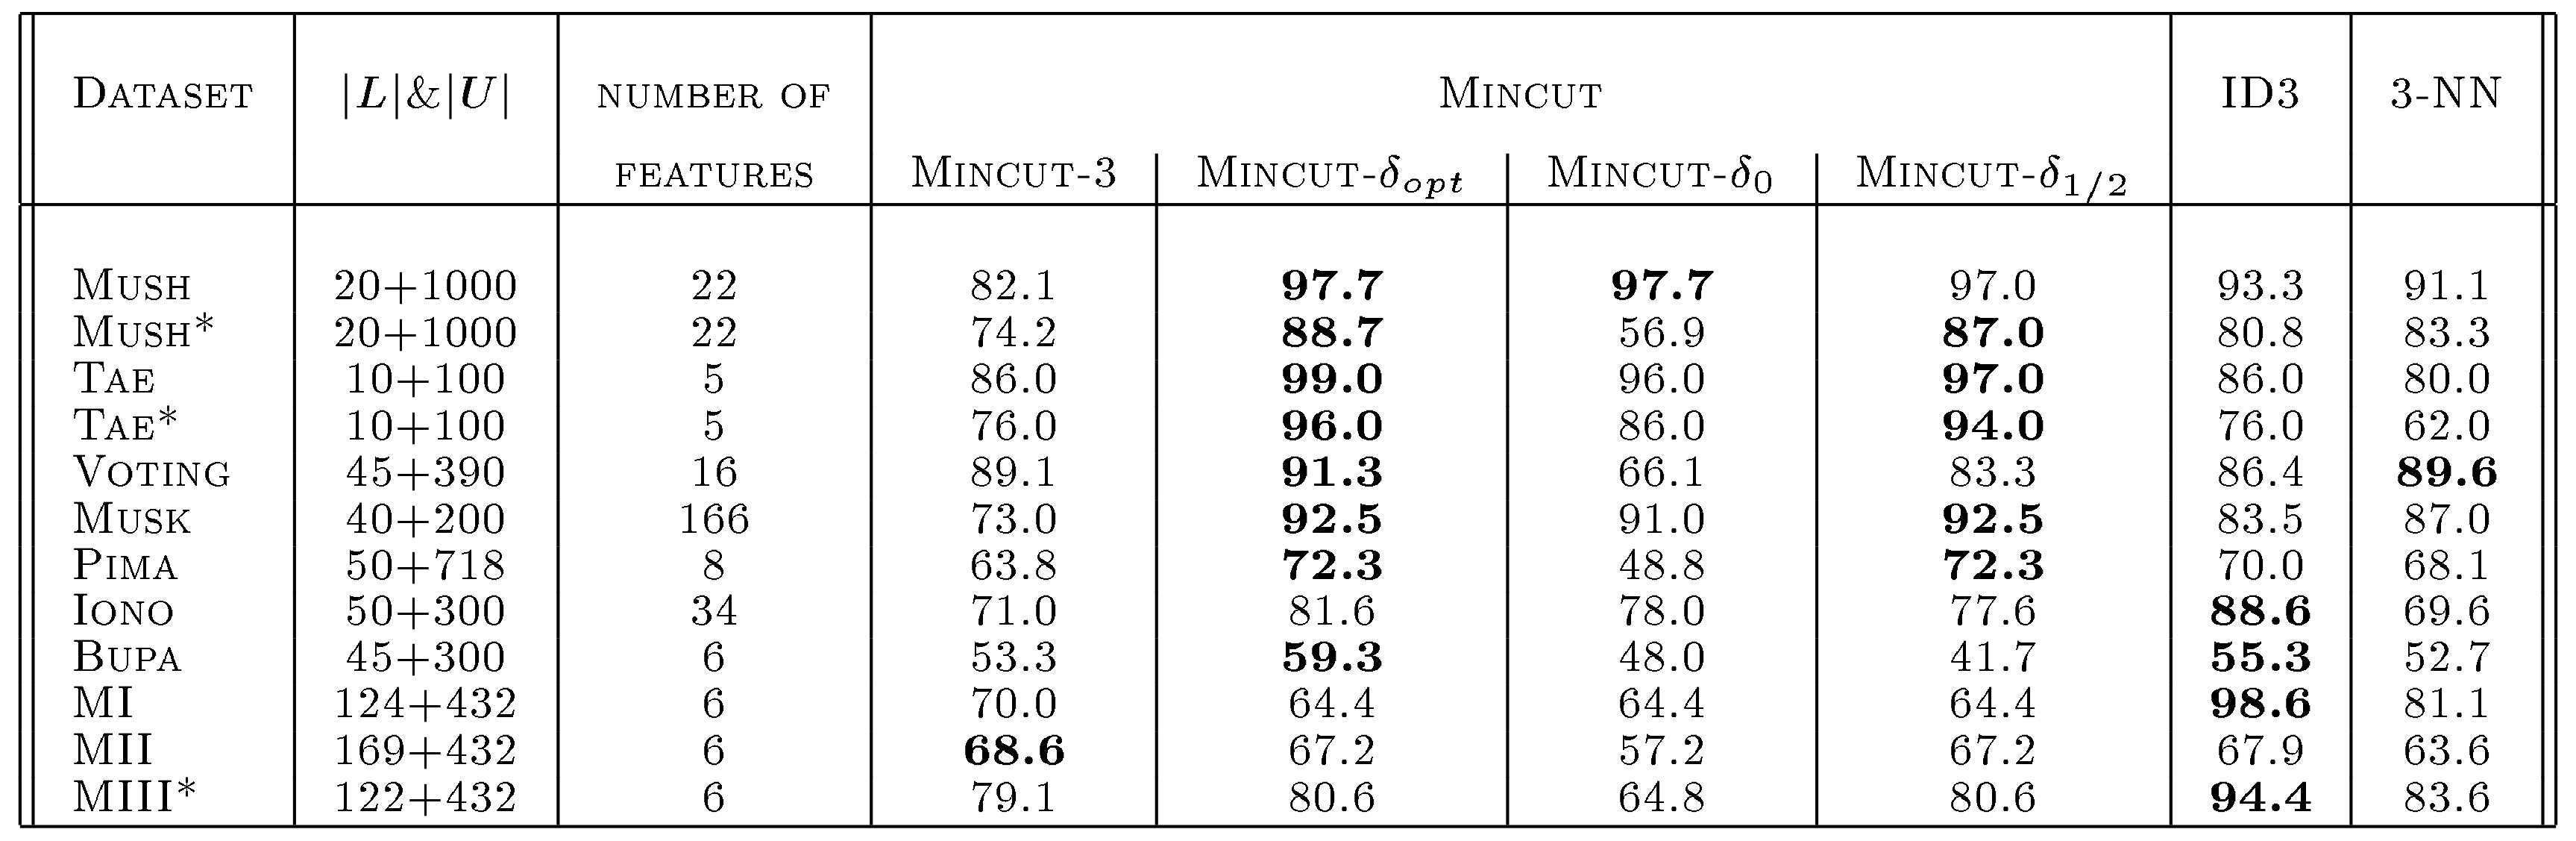
\includegraphics[width=1\textwidth]{mincut-comp}
        \end{center}
        \caption{Mincut com alguns valores para $\delta$ e comparação com outros métodos.}
      \end{figure}
    }

    \frame
    {
      \frametitle{Mincut - Desempenho Comparativo (2)}
      \begin{figure}[!h]
        \begin{center}
                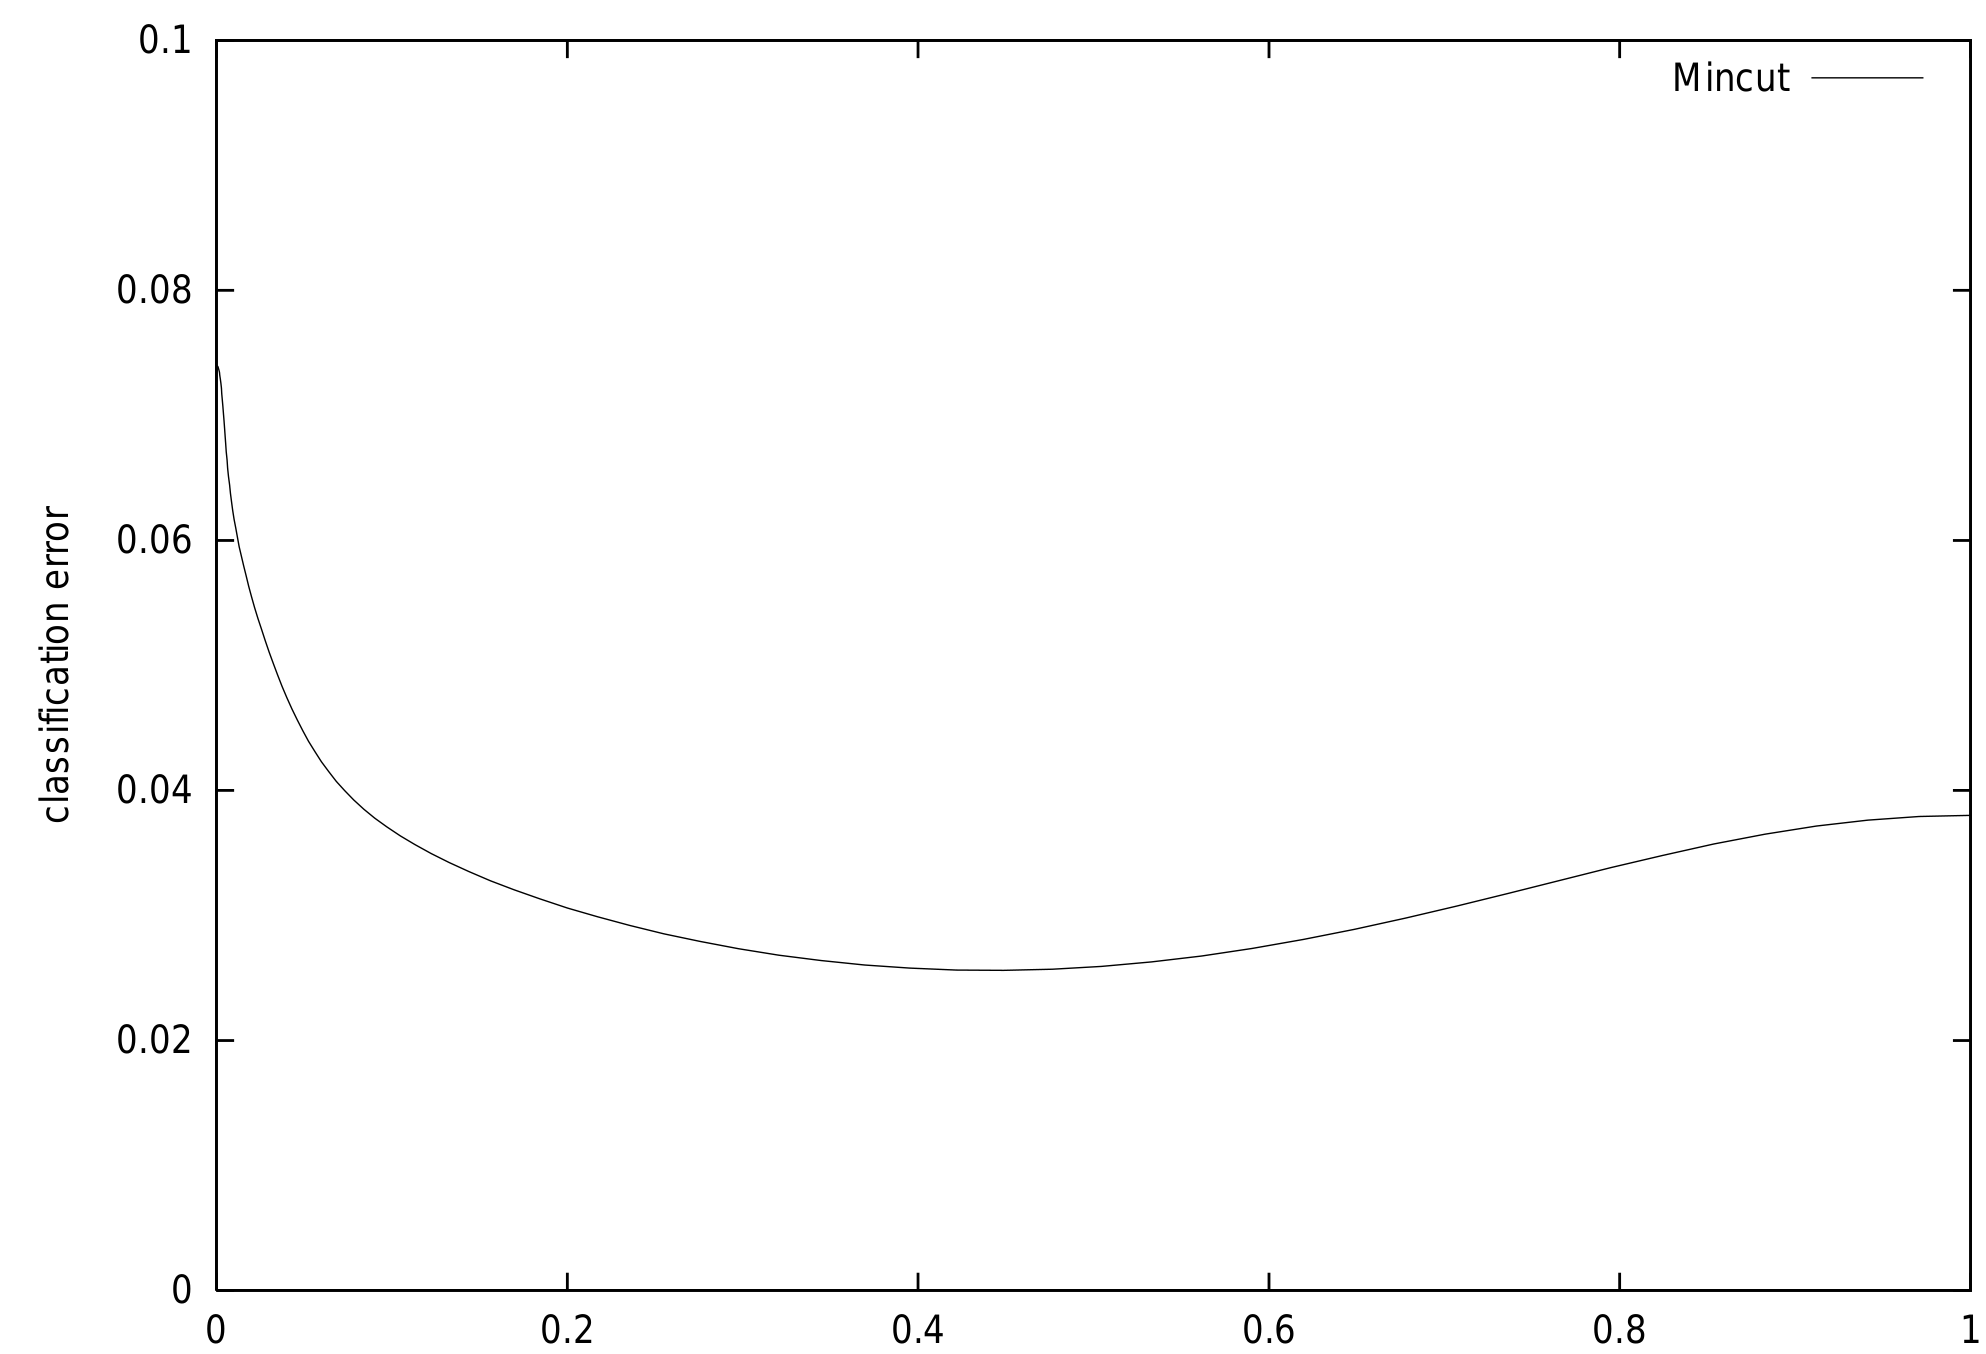
\includegraphics[width=.5\textwidth]{mincut-delta}
        \end{center}
        \caption{Variação do erro com o Delta.}
      \end{figure}
    }

    \frame
    {
      \frametitle{Mincut - Desempenho Comparativo (3)}
      \begin{figure}[!h]
        \begin{center}
                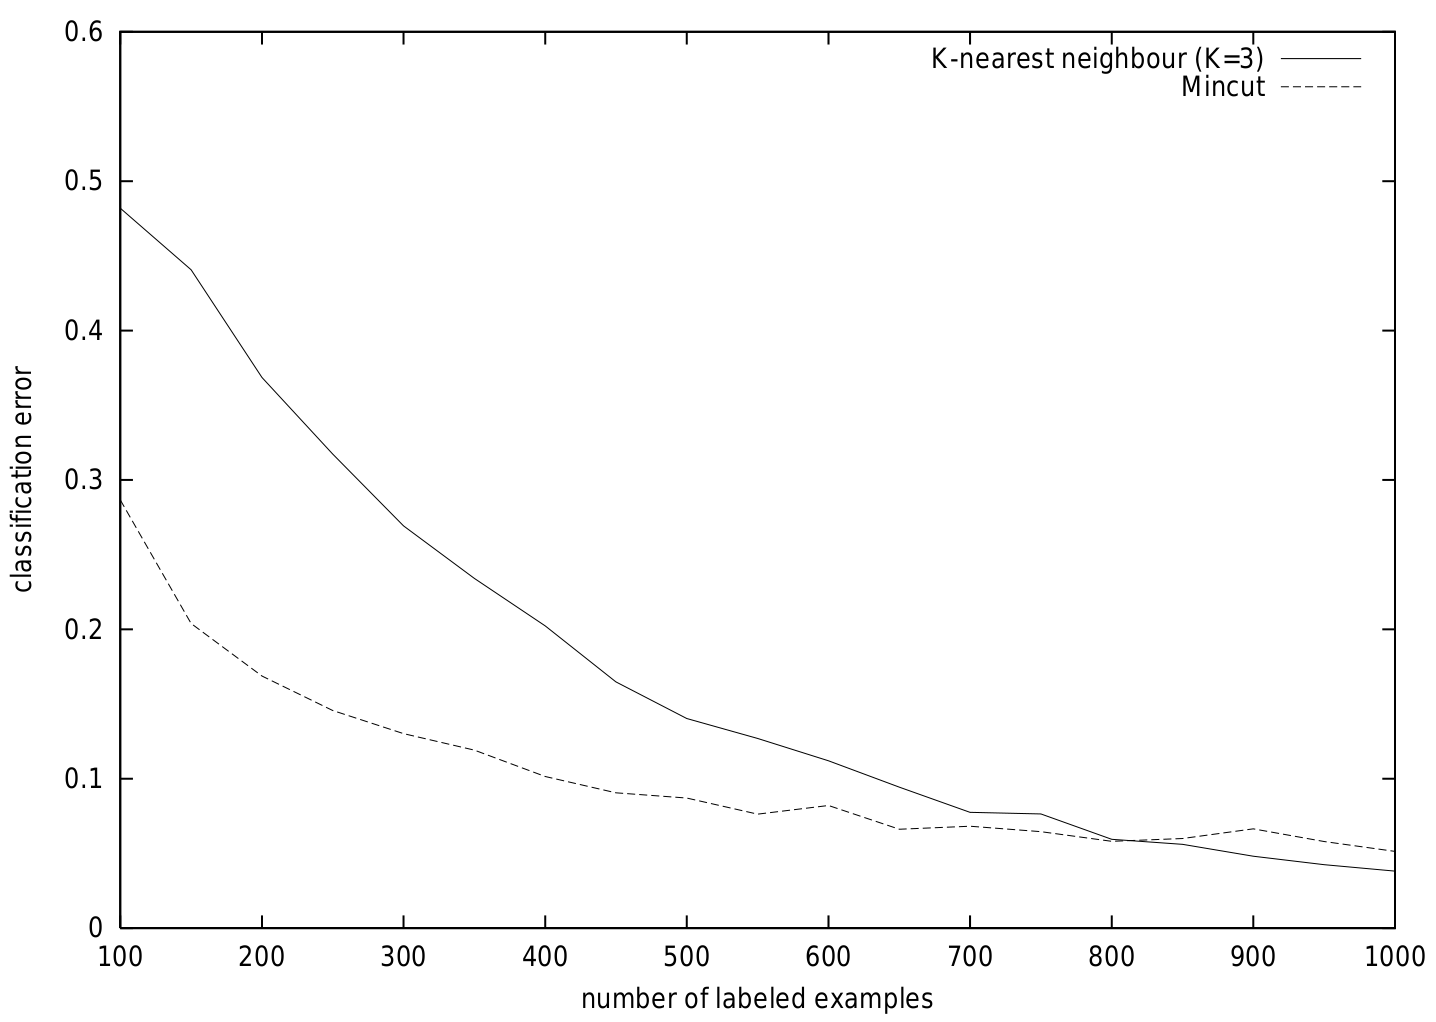
\includegraphics[width=.5\textwidth]{mincut-erro-l}
        \end{center}
        \caption{Comparação do erro entre mincut e kNN com a variação de exemplos rotulados $\delta_{opt}$.}
      \end{figure}
    }

    \frame
    {
      \frametitle{Mincut - Desempenho Comparativo (4)}
      \begin{figure}[!h]
        \begin{center}
                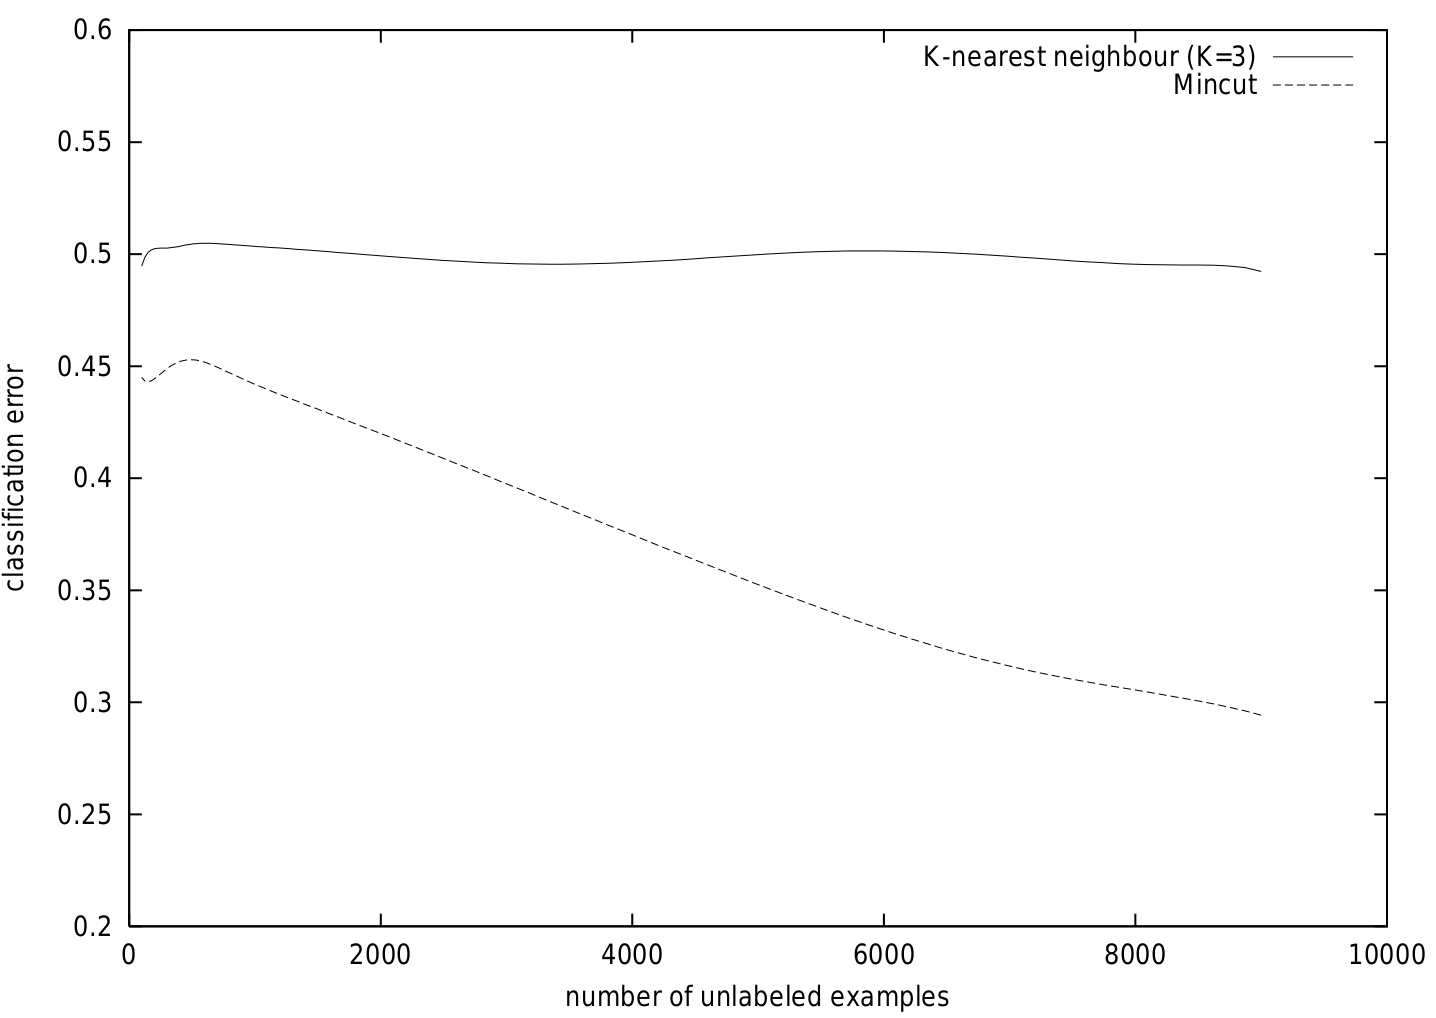
\includegraphics[width=.8\textwidth]{mincut-erro-u}
        \end{center}
        \caption{Comparação do erro entre mincut e kNN com a variação de exemplos não rotulados $\delta_{opt}$.}
      \end{figure}
    }

  \section{Conclusão}
    \frame
    {
      \frametitle{Conclusão}
      \begin{itemize}
        \item Com segurança se as classes são clusterizadas entre si. 
        \item Na falta de dados rotulados
        \item Seguindo a distribuição dos dados evitam o critério único da proximidade dos dados rotulados.
        \item Melhor que o kNN para os casos que vimos.
        \item Complexidade simples-moderada.
      \end{itemize}
    }

    \section{Principais Referências}
    \frame
    {
      \frametitle{Referências Principais}
      \begin{itemize}
        \item Zhu, X. and Lafferty, J. and Rosenfeld, R. "Semi-supervised learning with graphs.", 2005
        \item Zhu, X. and Ghahramani, Z., "Learning from labeled and unlabeled data with label propagation.", 2002
        \item Blum, A. and Chawla, S., "Learning from labeled and unlabeled data using graph mincuts", 2001
      \end{itemize}
    }

    \frame
    {
      \frametitle{FIM.}

        FIM.

    }
\end{document}
